\documentclass[a4paper]{article}

\usepackage[english]{babel}
\usepackage[bitstream-charter]{mathdesign}
\usepackage[T1]{fontenc}
\usepackage{graphicx}


\begin{document}
\selectlanguage{english}

\title{Comparative Programming Languages\\
Assignment $^{\#}$2: Domain Specific Language}
\author{Glenn Croes \and Philippe De Croock \and Thomas Winant}
\date{11 January, 2012}

\maketitle

\section{Domain description}
\label{sec:domain-description}

% An elaboration on elements of the domain that were missing or needed to be improved, plus justification for any choices made.


% Vluchtnummer per vlucht, onafhankelijk van het vliegtuig
% Schedule-schedulItem kan mss nog worden verbeterd
% tijdstip per flight
% elke 1..* ipv 0..* in ons systeem
% Each flight of a certain flight template happens with the same airplane model

\newcommand{\field}[1]{\emph{#1}}

\section{Domain analysis}
\label{sec:domain-analysis}
% A brief breakdown of the elements in your domain and how they relate to each other. This could be a formal meta-model, but could also be textual description.

\begin{figure}[ht!]
  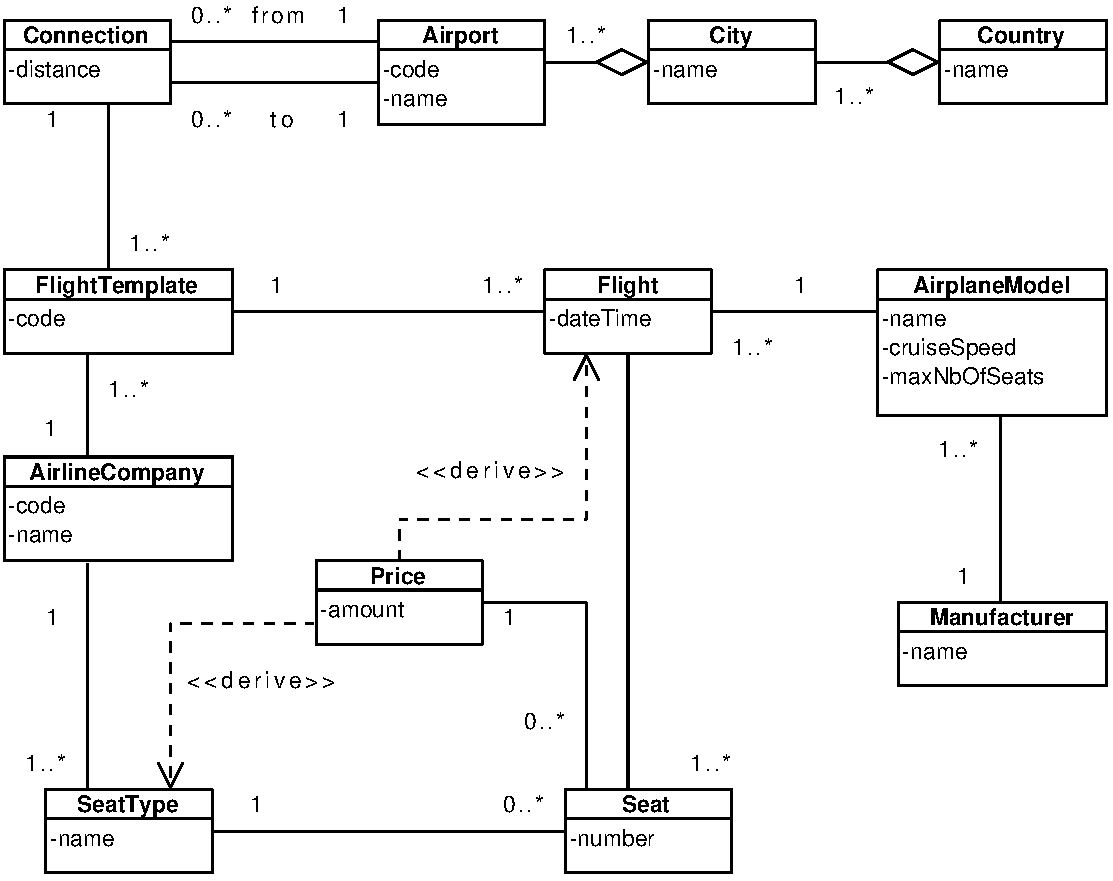
\includegraphics[width=1.0\textwidth]{../analysis/domainModel.pdf}
  \caption{Domain Model}\label{fig:domain-model}
\end{figure}

\paragraph{Country}
A \field{Country} has a name and represents a sovereign nation.
\paragraph{City}
A \field{City} has a name and is located in a country.
\paragraph{Airport}
An \field{Airport} is located in a city.
It has a name and is uniquely identified by its 3 capital letter code.
It is possible for a city to have multiple airports.
\paragraph{Connection}
A \field{Connection} represents a flight link between two airports.
The distance in kilometers of the connection is stored.
A connection must be between two different airports.
\paragraph{AirlineCompany}
An \field{AirlineCompany} provides air transport services for passengers.
It has a name and is uniquely identified by a 2 or 3 capital letter code.
\paragraph{Manufacturer}
A \field{Manufacturer} is a business engaged in manufacturing airplanes.
Only the name of the manufacturer is relevant in our domain.
\paragraph{AirplaneModel}
An \field{AirplaneModel} is manufactured by a manufacturer.
It has a name and cruise speed.
The maximum number of seats that can be installed in the airplane model is stored too.
\paragraph{FlightTemplate}
A \field{FlightTemplate} describes a template for flights.
Each flight template is denoted by a code consisting of the airline code followed by 3 or 4 digits.
Airline companies define flight templates for certain connections.

% TODO
% recurs at the same time one or more
% days per week
% flight that recurs at the same time one or more
% days per week. (Some flight takes place on just one day per week, others a
% couple of days per week, others every day.)
% To specify a specific flight, the date is also required.

% It is probably a good idea to separate the information about the flight and the
% ‘template’ describing flights. The ‘template’ includes the flight code, but the
% actual flight details include the date.

\paragraph{Flight}
A \field{Flight} is an instantiation of a flight template at a particular date and time.
As they are dependent on a flight template, flights are specific to airline companies.
A flight will happen with a certain airplane model.
\paragraph{SeatType}
A \field{SeatType} is used to define seat classes, for instance business and economy are two seat types.
Only the name of the seat type is stored.
Different airline companies can reuse the same seat types.
\paragraph{Seat}
A \field{Seat} represents a seat on a flight.
A seat has a seat number that is unique on the airplane.
\paragraph{Price}
Every seat on a flight has a \field{Price}.
The price depends on the flight and the seat type.
This means that two seats, both of the same seat type and both on flights that follow the same template, can have different prices on different dates.


\section{Design description}
\label{sec:design-description}


\begin{figure}[ht!]
  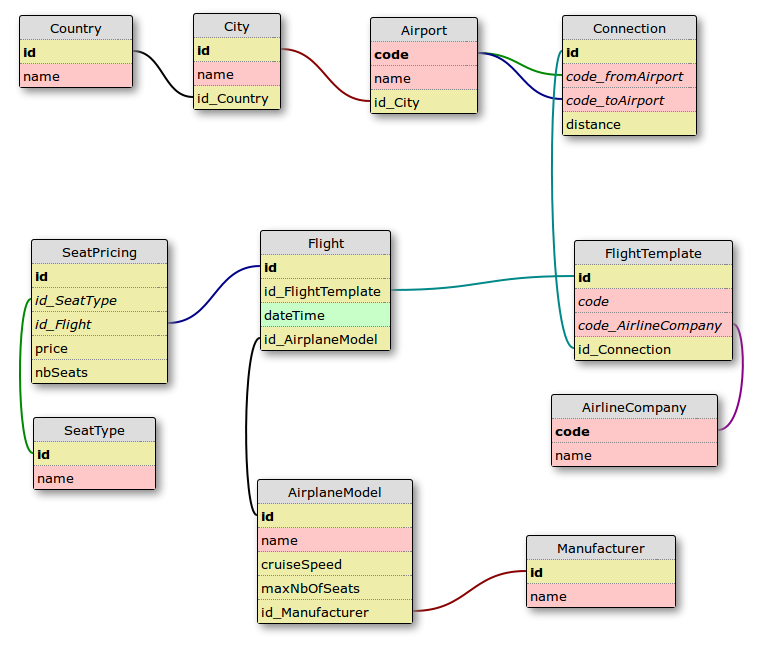
\includegraphics[width=1.0\textwidth]{../analysis/dbtables-diagram.png}
  \caption{Database Tables}\label{fig:database-tables}
\end{figure}


% A description of the semantic model underlying the DSL, along with a description of the constructs of your DSL.

\section{Implementation overview}
\label{sec:implementation-overview}

% A general overview of the implementation approach, including a description of the API upon which it is based and any tricky implementation techniques employed. Some justification of the chosen implementation language needs also to be provided.

\section{DSL Implementation}
\label{sec:dsl-implementation}

% The code implementing your DSL and any libraries on which it is based.

\section{Example DSL program(s)}
\label{sec:example-dsl-programs}

% Some example DSL programs to illustrate how your DSL is to be used.

\section{Guide}
\label{sec:guide}

% to use A short description of how to compile and run your DSL and a guide to the structure of the submitted files.



\end{document}


%%% Local Variables:
%%% mode: latex
%%% ispell-local-dictionary: american
%%% TeX-master: t
%%% End:
